\chapter{Analýza}\label{analysis}

Tato kapitola nejprve blíže popisuje formát a mechaniky originální hry a dále pojednává o postupech a řešeních použitých 
při implementaci nového enginu. Jsou zde popsány jak slepé a nevhodné návrhy, tak návrhy, které se ukázaly 
jako nejvhodnější řešení.

Pro splnění práce bylo v prvé řadě zapotřebí získat vstupní data originální hry Dungeon Master. Nejdůležitější data 
jsou obsažená ve dvou souborech: \ccc{DUNGEON.DAT} a \ccc{GRAPHICS.DAT}. První z nich obsahuje definice herních úrovní a seznamy 
použitých předmětů, přepínačů a nepřátelských entit. Druhý z nich obsahuje konkrétní vlastnosti objektů a entit použitých v prvním souboru. 
Soubor \ccc{GRAPHICS.DAT} pak také obsahuje definicí akcí, vlastnosti kouzel, textury, atd. Později se ukázalo, že pouze data hry nebudou
pro implementaci většiny funkcí dostačující -- jedná se například o přesný způsob získávání dovedností šampionů, 
vyvolávání kouzel nebo provádění akcí. Dalším zdrojem jsou proto dekompilované zdrojové kódy \cite{DMDecompilation} originální hry v jazyce C s archaickou konvencí Kernighan \&
Ritchie.\footnote{
Brian Kernighan a Dennis Ritchie jsou autoři první verze jazyka C, jehož neformální specifikaci popsali v první edici knihy \textit{The C Programming Language} \cite{krc}.
Podle iniciálů autorů této knihy je tato první verze jazyka známa jako K\&R C. Mezi největší specifika K\&R C patří:

\begingroup
\renewcommand{\theenumi}{\Alph{enumi}}
\begin{enumerate}
\item\label{declaration} deklarace funkcí nespecifikuje parametry a není prováděna jejich kontrola,
\item\label{void} funkce nemají návratový typ \ccc{void},
\item\label{params} při definici funkce jsou typy parametrů specifikovány na separátních řádcích za hlavičkou funkce,
\item\label{locals} lokální proměnné funkcí jsou deklarovány na začátku bloku funkce.
\end{enumerate}
\endgroup


Ukázka kódu: \newline
\begingroup
\fontfamily{lmtt}\selectfont
//declaration\newline
typedef int VOID;					// viz bod \ref{void}\newline
VOID write\_sorted();				// viz bod \ref{declaration}\newline
\newline
//definition\newline
VOID write\_sorted(first, second)	// viz bod \ref{params}\newline
int first;\newline
int second;\newline
\{\newline
\hspace*{4em}	int min;						// viz bod \ref{locals}\newline
\hspace*{4em}	int max;\newline
\newline
\hspace*{4em}	printf("We are about to find out sorted sequence\textbackslash n");\newline
\newline
\hspace*{4em}	if(first < second)\{\newline
\hspace*{4em}\hspace*{4em}		min = first;\newline
\hspace*{4em}\hspace*{4em}		max = second;\newline
\hspace*{4em}	\} else \{\newline
\hspace*{4em}\hspace*{4em}		min = second;\newline
\hspace*{4em}\hspace*{4em}		max = first;\newline
\hspace*{4em}	\}\newline
\hspace*{4em}	printf("Sorted values are (\%d, \%d)\textbackslash n", min, max);\newline
\}
\endgroup } 
Tyto zdrojové kódy jsou často špatně srozumitelné, nicméně potřebné informace pro dokončení této práce se z nich podařilo získat.

Pro detailnější popis dat Dungeon Masteru si bude dobré nejprve ujasnit vlastnosti a schopnosti šampionů.
Každý šampion má následující vlastnosti:\label{properties-skills}
\begin{itemize}
\item \xxx{Zdraví} (Health) -- určuje kolik útoku šampion vydrží, než zemře,
\item \xxx{Výdrž} (Stamina) -- určuje kolik akcí je schopen šampion vykonat, než se unaví, 
\item \xxx{Mana} (Mana) -- reprezentuje magickou energii pro vyvolávání kouzel, 
\item \xxx{Zatížení} (Load) -- určuje maximální hmotnost, kterou je šampion schopen unést,
\item \xxx{Síla} (Strength) --  hodnota je používána pro výpočet zranění, síly hodu předmětů a maximální výše zatížení,
\item \xxx{Obratnost} (Agility) -- zvyšuje pravděpodobnost zásahu nepřítele a pomáhá se vyhnout nepřátelským útokům,
\item \xxx{Moudrost} (Wisdom) -- je vlastnost důležitá pro kouzelníky a kněze, určuje rychlost obnovy many,
\item \xxx{Vitalita} (Vitality) -- určuje rychlost obnovy zdraví a výdrže,
\item \xxx{Odolnost proti magii} (Magic Defense) -- snižuje účinnost magických útoků,
\item \xxx{Odolnost proti ohni} (Fire Defense) -- snižuje účinnost ohnivých útoků,
\item \xxx{Jídlo a Voda} (Food and Water) -- pomocí těchto hodnot je obnovována výdrž a zdraví,
\item \xxx{Štěstí} (Luck) -- zvyšuje či snižuje pravděpodobnost provedení akce.
\end{itemize}

Každý šampion má ve hře čtyři základní dovednosti: bojovník, ninja, kněz a kouzelník.
Kromě základních dovedností má šampion ještě šestnáct skrytých dovedností, které nejsou hráči zobrazeny.
Každá z těchto skrytých dovedností náleží k nějaké ze základních dovedností.
Jak moc je daný šampion zkušený v dané dovednosti, určuje úroveň dovednosti. 
Tuto úroveň lze navyšovat pomocí zkušeností, které lze získat souboji nebo prováděním akcí. Každá
akce pak může navyšovat zkušenosti pro jinou dovednost. Pokud jsou v některé ze skrytých dovedností 
získány zkušenosti, dostane odpovídající zkušenosti i její základní dovednost. Po získání dostatečného
počtu zkušeností v nějaké dovednosti, získá šampion v této dovednosti novou úroveň. Nová úroveň potom
navýší určité vlastnosti šampiona. Přesné hodnoty potřebných zkušeností a navyšovaných vlastností pro 
odpovídající dovednosti jsou pevně stanovené ve zdrojových kódech hry.

\section{Data s herními úrovněmi -- \ccc{DUNGEON.DAT}}\label{dungeon-objects}

Originální hra má herní úrovně definované v binárním souboru \ccc{DUNGEON.DAT}. Formát tohoto souboru nebyl tvůrci nikdy zveřejněn,
nicméně kolem hry se vytvořila početná komunita, která k němu dokumentaci \cite{TechnicalDocumentationFontanel05} vytvořila.
Tuto dokumentaci jsme použili k porozumění obsahu souboru. Následuje stručný popis zmíněného souboru, pro 
kompletní dokumentaci navštivte přímo stránky dokumentace.

Soubor \ccc{DUNGEON.DAT} obsahuje jednotlivé herních úrovně a objekty v nich obsažené.
 Formát souboru lze rozdělit do následujících bloků \cc{dungeon-general-format}:
\begin{itemize}
\item Hlavička souboru -- obsahuje velikost jednotlivých bloků souboru nebo velikost seznamů objektů.
\item Vlastnosti herních úrovní -- mezi tyto vlastnosti patří rozměry dané úrovně, tj. počet dlaždic na šířku a výšku. Dále
	definuje obtížnost úrovně, která je použita pro výpočet získaných zkušeností nebo zdraví nepřátelských entit. Každá úroveň má
	také určené použité podmnožiny dekorací na zdech, dveřích a přepínačích. Dekorace jsou v originální hře identifikovány čísly, která
	jsou napevno zabudovaná v kódu hry. Některé dekorace tak mohou mít navíc speciální význam, který je enginem identifikován
	pouze podle zmíněného číselného identifikátoru. Jedná se například o dekorace s výklenky, které mohou být umístěné na zdech.
	V tomto případě originální herní engine rozpozná, že lze na dané místo vkládat předměty. 
\item Textová data -- obsahuje všechny texty ve hře.
\item Seznamy obecných objektů -- mezi tyto objekty patří, dveře, teleporty, popisky na zdech a přepínače.
\item Seznamy předmětů -- jsou to předměty, které se dají v herních úrovních sbírat a používat. 
\item Data úrovní -- obsahují data pro každou dlaždici v každé úrovni.
\end{itemize}
Jednotlivé části souboru budou popsány detailněji v následujících sekcích.

\imgx{dungeon-general-format}{Ilustrace formátu souboru \ccc{DUNGEON.DAT}.}


\subsection{Dlaždice (Tiles)}

Dlaždice se dělí na několik typů a pomocí přepínačů jim lze zaslat zprávu, na kterou mohou reagovat. Zpráva obsahuje akci a datovou položku. 
Akce dlaždici říká, zda se má aktivovat či deaktivovat. Co daná datová položka znamená si určuje každý typ cílové dlaždice sám. 
Originální hra pak pracuje s následujícími typy dlaždic:
\begin{itemize}
\item \xxx{Zeď} (Wall) -- zajišťuje zobrazování stěn a nelze na ni vstoupit. Pro každou stěnu  (sever, východ, jih, západ -- viz obr. \ref{wall:analyza}) dlaždice \xxx{zdi}
	je určeno, zda může mít tzv. náhodnou dekoraci. Pokud ji může mít, engine podle náhodného generátoru
	určí, jaká to bude (případně žádná). Každá strana \xxx{zdi} může obsahovat přepínač, který si může do \xxx{zdi} uložit předměty.
	Pokud má některá strana dekoraci výklenku, jsou v něm zobrazeny předměty uložené ve \xxx{zdi}.
	Na stěnách \xxx{zdi} ještě mohou být popisky, které lze zobrazovat nebo skrývat pomocí zaslání zprávy. Aktivační zpráva 
	popisek zviditelní a deaktivační skryje. Datová položka zprávy zde určuje, pro kterou ze stěn \xxx{zdi} je zpráva určena.

\item \xxx{Podlaha} (Floor) -- Po těchto dlaždicích se hráč běžně pohybuje se svoji skupinou. Obdobně jako u stran \xxx{zdí} může definovat,
	zda zobrazuje na podlaze náhodnou dekoraci. Podlaha dále může mít nášlapný přepínač. Dlaždice obsahuje čtyři pozice,
	na které lze pokládat předměty. Tyto pozice vzniknou rozdělením plochy dlaždice na čtvrtiny \cc{floor:analyza}.


\item \xxx{Jáma} (Pit) -- \xxx{Jáma} může být buď otevřená nebo zavřená. Nicméně lze na ni vždy vstoupit, a pokud je otevřená, 
	hráč spadne se svoji skupinou o úroveň níže. Pád může být i přes několik úrovní. Živé objekty pak po
	dopadu obdrží zranění. Přijmutím aktivační zprávy se jáma otevře a deaktivační se zavře.

\item \xxx{Schody} (Stairs) -- Po této dlaždici se může hráč dostat o úroveň výše resp. níže.

\item \xxx{Dveře} (Door) -- Na těchto dlaždicích je vždy objekt dveře. Na dlaždici lze vstoupit pouze v případě, že jsou dveře
	otevřeny. Otevření je možné provést aktivační zprávou či pomocí tlačítka -- pokud ho samotné dveře obsahují. 
	Některé dveře lze také rozbít útokem, to si ale definuje již samotný objekt dveří.

\item \xxx{Teleport} (Teleporter) -- Tyto dlaždice obsahují objekt teleport, který určuje, které objekty dokáže přenést. Mohou to být
	předměty, hráčova skupina nebo nepřátelské entity. Po vstupu resp. vložení objektu na dlaždici, je objekt teleportován, pokud
	je odpovídajícího typu. Příjem aktivační resp. deaktivační zprávy aktivuje resp. deaktivuje teleport.

\item \xxx{Iluze zdi} (Trick wall) -- Tato dlaždice může být buď iluze zdi a nebo otevíratelná zeď. V obou případech je vizuálně neodlišitelná
	od dlaždice typu \xxx{zeď}. V prvním případě je možné na dlaždici vstoupit vkročením do zdi. V druhém případě lze
	zeď odstranit pomocí zaslání odpovídající zprávy na dlaždici. Aktivační zpráva otevře zeď, deaktivační zavře.
\end{itemize}

	\begin{figure}[H]
    \centering
    \begin{subfigure}[b]{0.45\textwidth}
        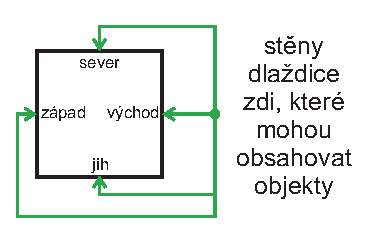
\includegraphics[width=\textwidth]{./img/DM-wall-sides}
        \caption{Dlaždice zeď -- stěny.}
        \label{wall:analyza}
    \end{subfigure}
    \begin{subfigure}[b]{0.45\textwidth}
        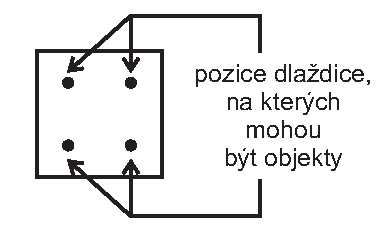
\includegraphics[width=\textwidth]{./img/DM-floor-spaces}
        \caption{Dlaždice podlaha -- pozice.}
        \label{floor:analyza}
    \end{subfigure}
    \caption{Možné pozice pro uložení objektů na dlaždici.}\label{tile-positions:analyza}
\end{figure}

Samotné úrovně jsou pak vždy definovány následujícími seznamy v tomto pořadí:
\begin{itemize}
\item seznam dlaždic -- seřazeny po sloupcích dané úrovně,
\item seznam dekorací příšer,
\item seznam dekorací zdí, 
\item seznam dekorací podlah.
\end{itemize}
Počty jednotlivých dekorací a dlaždic jsou popsány ve vlastnostech úrovní.

\subsection{Textová data}

V binárním souboru jsou často data uložena po slovech procesoru, které v tomto případě mají velikost dvou bajtů. 
V této části souboru jsou uložena data s použitými texty ve hře. Tyto texty používají speciální kódování,
kdy jednotlivé znaky jsou uloženy do slov  (těch procesorových) a každé toto slovo obsahuje tři znaky. Všechny 
texty jsou pak uloženy za sebou v jednom bloku a ke konkrétním textům je přistupováno přes offsety počtu bajtů
od začátku textových dat. Přesný popis je opět k nalezení v komunitní dokumentaci \cite{TechnicalDocumentationFontanel05}.

\subsection{Objekty}

Tyto objekty uložené v souboru \ccc{DUNGEON.DAT} tvoří jednotlivé instance. Odpovídající typy
k těmto instancím jsou potom spolu s jejich neměnnými vlastnostmi uloženy v souboru \ccc{GRAPHICS.DAT},
jehož obsah si rozebereme v následující sekci \ref{dungeon-properties}. Tyto typy se pak ještě dělí do kategorií popsaných dále v této sekci.
Pro určení konkrétního typu má potom každá instance uložen index typu v dané kategorii \cc{instance-type}.
Objekty reprezentující instance obsahují pouze vlastnosti, které jsou rozdílné pro každou konkrétní instanci.

\imgx{instance-type}{Ilustrace vztahu instancí a typů.}

\subsubsection{Identifikátory}

Ke každé instanci objektu existuje unikátní identifikátor, který se skládá z následujících částí:
\begin{itemize}
\item Pozice -- lze buď interpretovat jako světovou stranu, nebo 
	umístění na dlaždici, jedná-li se o podlahu.
\item Kategorie typu objektu -- pro každou kategorii existuje
	v souboru \ccc{DUNGEON.DAT} seznam jejich instancí.
\item Index -- určuje index objektu v seznamu instancí jeho kategorie.
\end{itemize}

Tyto identifikátory se dají chápat jako reference na konkrétní instance objektů \cc{identifier-linklist},
pomocí nichž jsou vytvořeny spojové seznamy. Každá dlaždice pak specifikuje, zda může mít spojový seznam.
Seznam objektových identifikátorů obsahuje první identifikátory spojových seznamů na dlaždicích, které 
je mají. Seznam je uspořádaný pro všechny dlaždice od první do poslední úrovně, vždy po sloupcích odshora dolů \cc{identifier-list}.

\imgx{identifier-linklist}{Ilustrace obsahu identifikátoru a jeho využití ve spojových seznamech.}
\imgx{identifier-list}{Ilustrace uspořádání prvních objektových identifikátorů dlaždic.}

\subsubsection{Předměty}\label{grabable-items}

Předměty jsou objekty, které lze sbírat, používat nebo ukládat k šampionům.
Dělí se do následujících kategorií:
\begin{itemize}
\item \xxx{Zbraně} (weapons) -- lze je vložit šampionům do ruky a ti pak s nimi mohou bojovat.
\item \xxx{Oblečení} (clothes/armor)-- lze jím obléknout šampiony, a tak zvýšit jejich odolnost.
\item \xxx{Svitky} (scrolls) -- obsahují text, který může hráči usnadnit hru.
\item \xxx{Lektvary} (potions) -- dělí se na lektvary modifikující šampionovi schopnosti a na lektvary provádějící nějaké
	akce -- např.: výbuch. Každá instance má vlastnost určující sílu efektu.
\item \xxx{Kontejnery} (containers) -- mohou obsahovat další předměty.
\item \xxx{Různé} (miscellaneous)-- v této kategorii je například jídlo nebo různé předměty, s kterými nelze provádět žádné akce.
\end{itemize}

\subsubsection{Ostatní objekty}
Tyto objekty slouží jako pomocné objekty pro dlaždice a dělí se do následujících kategorií:

\begin{itemize}
\item \xxx{Dveře} (door) -- můžou být pouze na dlaždici typu \xxx{dveře} a obsahují informace, zda-li jsou dveře rozbitelné a jestli 
	mají tlačítko, kterým je lze otevřít.
\item \xxx{Teleport} (teleporter) -- může být pouze na dlaždici typu \xxx{teleport} a definuje cílovou dlaždici a kategorii objektů, které je schopen teleportovat.
\item \xxx{Textové popisky} (texts) -- mohou být pouze na dlaždici typu \xxx{zeď} a obsahují odkaz na konkrétní text do textový dat.
\item \xxx{Skupina nepřátelské entity} (creatures) -- definuje skupinu nepřátelských entity na dlaždici, jejich počet, rozmístění na dlaždici a předměty, které lze získat jejich zabitím.
\item \xxx{Senzory} (sensors/actuators) -- vytvářejí základní mechaniky herních úrovní. Senzory mají daný číselný typ, pomocí kterého hra 
	určí, jakým způsobem je možné senzor
	aktivovat. Po aktivaci senzor buď může provést lokální akci, nebo odeslat zprávu s akcí na vzdálenou 
	dlaždici. Přepínače se pak typicky skládají z několika senzorů. Více o přepínačích a senzorech bude zmíněno
	v sekci \ref{actuator-analyza}. 
\end{itemize}

\section{Data s vlastnostmi objektů -- \ccc{GRAPHICS.DAT}}\label{dungeon-properties}

Soubor \ccc{GRAPHICS.DAT} obsahuje textury dekorací, vlastnosti předmětů a objektů, definici akcí a kouzel.
Formát tohoto souboru nebyl tvůrci uveřejněn, avšak komunitě se opět podařilo data
vyextrahovat. K některým částem také existuje komunitní dokumentace \cite{DMGraphicsDAT}, 
nicméně není ucelená jako v případě dokumentace souboru \ccc{DUNGEON.DAT}. Zároveň 
jsou vyextrahovaná data zveřejněna na webu v HTML formátu (\cite{DMActions}, \cite{DMItems}, \cite{DMItemDescriptors}, \cite{DMSpells}, \cite{DMCreatures}). Z toho důvodů jsme se rozhodli 
pro využití již extrahovaných dat v HTML formátu. Dále následuje podrobnější popis využitého obsahu souboru.

\subsection{Akce a komba}\label{action-combos}

S předměty je možné provádět akce. Množina akcí pro daný předmět se nazývá kombo a obsahuje 
až tři akce. Ve hře je k dispozici 44 akcí a stejný počet komb. Kompletní seznam jednotlivých
akcí a komb lze nalézt v komunitní dokumentaci \cite{DMActions}. Zde si popišme alespoň jejich vlastnosti.

\medskip

Vlastnosti akcí jsou:
\begin{itemize}
\item \xxx{název} (name) -- textový popis akce ve hře,
\item \xxx{zkušenosti} (experience gain) -- počet zkušeností získaných po provedení akce,
\item \xxx{dovednost} (skill) -- identifikátor dovednosti, která získá zkušenosti,
\item \xxx{obrana} (defense modifier) -- modifikátor obrany při používání akce,
\item \xxx{výdrž} (stamina) -- modifikátor výdrže nutné pro provedení akce, 
\item \xxx{pravděpodobnost provedení akce} (hit probability),
\item \xxx{zranění} (damage) -- modifikátor pro výpočet konečného zranění nepřítele, 
\item \xxx{únava} (fatigue) -- doba, po kterou nelze provádět žádné akce. 
\end{itemize}

\medskip

Vlastnosti pro každou akci komba jsou:
\begin{itemize}
\item index akce ze seznamu akcí (action index), 
\item úroveň dovednosti (skill level) -- minimální úroveň dovednosti pro úspěšné provedení akce. 
\end{itemize}


\subsection{Předměty}\label{item-descriptors}

Ke každému typu předmětu existují v tomto souboru popisovače vlastností \cite{DMItemDescriptors}.
Pro každý předmět jsou definovány následující vlastnosti:  
\begin{itemize}
\item \xxx{globální identifikátor} (global item index) -- unikátní identifikátor, který je použit k identifikaci konkrétního typu předmětu například v přepínačích,
\item \xxx{index útočného komba} (attack combo),
\item \xxx{lokace} (carry location) -- místo, na kterou část těla, nebo do kterého inventáře šampiona lze předmět vložit,
\item \xxx{index v kategorii} (index in its category) -- index typu předmětu v dané kategorii.
\end{itemize}

Globální identifikátor lze z instance předmětu získat pomocí jeho kategorie a indexu typu předmětu,
který má každá instance předmětu. Každý předmět má také definovanou hmotnost. Zbraně a oblečení mají navíc
definované následující vlastnosti, jejichž hodnoty lze nalézt v komunitní dokumentaci \cite{DMItems}.

\medskip

Zbraně:
\begin{itemize}
\item \xxx{poškození} (damage) -- hodnota zranění aplikovaná při útoku na nepřítele,
\item \xxx{kinetická energie} (energy) -- hodnota udává, jak daleko lze zbraň hodit,
\item \xxx{střelné poškození} (shoot damage) -- hodnota dodatečného poškození u střelných zbraní.
\end{itemize}

Oblečení:
\begin{itemize}
\item \xxx{síla brnění} (armor strength) -- obrana, kterou oblečení poskytuje, 
\item \xxx{odolnost proti útokům ostrými předměty} (sharp resistance). 
\end{itemize}

\subsection{Kouzla a symboly}\label{magic-symbols}

Další častí dat uložené v souboru \ccc{GRAPHICS.DAT} jsou vlastnosti kouzel. Pojď\-me si nejprve přiblížit,
jak se ve hře kouzla přesně vyvolávají. Každé kouzlo je složeno z několika symbolů, přičemž první 
z nich je speciální a jde o tzv. ,,power symbol". Power symbol určuje, jak bude celkové kouzlo silné.
Další symboly už určují konkrétní kouzlo. Každé vyvolání symbolu stojí šampiona \xxx{manu}. Po stanovení 
všech symbolů může šampion vyvolat samotné kouzlo. Vyvolání kouzla může selhat, pokud nemá šampion 
dostatečnou úroveň dovednosti vyžadované kouzlem. Datový soubor tedy obsahuje pro každý symbol při odpovídajícím
power symbolu množství potřebné many pro jeho vyvolání. Dále obsahuje následující vlastnosti kouzel \cite{DMSpells}:

\begin{itemize}
\item \xxx{Obtížnost} (Difficulty) -- modifikátor obtížnosti vyvolání kouzla,
\item \xxx{Doba trvání} (Duration) -- po tuto dobu nemůže šampion vyvolávat další kouzla,
\item \xxx{Úroveň dovednosti} (Skill level) -- postačující úroveň určité dovednosti pro úspěšné vyvolání kouzla.
\end{itemize}

\subsection{Nepřátelské entity}\label{properties-creatures}

Poslední částí obsaženou v souboru \ccc{GRAPHICS.DAT}, kterou jsme využili, jsou vlastnosti nepřátelských entit.
Následující výčet obsahuje vlastnosti, které implementuje nový engine. 
\begin{itemize}
\item \xxx{Doba pohybu} (Movement duration) -- doba, po které se entita rozhodne změnit pozici.
\item \xxx{Doba útoku} (Attack duration) -- doba, po které může entita provést útok.
\item \xxx{Síla brnění} (Armor) -- určuje odolnost proti útokům.
\item \xxx{Zdraví} (Base health) -- hodnota použitá pro výpočet zdraví nových nepřátelských entit.
\item \xxx{Síla útoku} (Attack power) -- hodnota pro výpočet útoku.
\item \xxx{Otrava} (Poison)  -- určuje, jak velkou otravu způsobí útok. 
\item \xxx{Obrana} (Defense) -- určuje obtížnost pro šampiona, se kterou je entita zraněna. 
\item \xxx{Detekce} (Detection range) -- určuje vzdálenost, na kterou detekuje nepřítele. 
\item \xxx{Odolnost proti ohni} (Fire resistance) -- odolnost proti kouzlům způsobující ohnivý útok.
\item \xxx{Odolnost proti jedu} (Poison resistance) -- odolnost proti kouzlům způsobující jedový útok.
\item \xxx{Pravděpodobnosti zranění částí těla} (Wounds) -- pravděpodobnost pro každou část těla nepřítele, s kterou ji entita zraní.
\end{itemize}

Celý seznam vlastností je možné nalézt v komunitní dokumentaci \cite{DMCreatures}.


\section{Parsování vstupních dat}\label{level-parsing}

V době implementace této části práce nebylo jasné, zda nalezená dokumentace \cite{TechnicalDocumentationFontanel05} bude dostatečná
pro splnění práce. Parser je proto oddělen od zbytku enginu do zvláštní assembly, která nereferencuje žádnou knihovnu
pro zobrazování grafiky. Cílem této assembly je tedy pouze převést struktury obsažené ve vstupních datech do odpovídajících
datových tříd v jazyce C\#. Tento balík dat se potom předá enginu, který z něj nich vytvoří herní úrovně. Toto schéma 
znázorňuje následující obrázek \ref{parser-preview}.

\imgx{parser-preview}{Ilustrace vztahu parseru vůči enginu.}

\subsection{Herní úrovně -- \ccc{DUNGEON.DAT}}\label{dungeon-parser}

Parsování herních úrovní je rozděleno do dvou fází. V první fázi probíhá transformace dat objektů \vref{dungeon-objects} ze souboru \ccc{DUNGEON.DAT}
 na odpovídající objekty v jazyce C\#. V druhé fázi jsou pak objekty z první fáze upraveny,
aby měly přehlednější strukturu. 


\subsubsection{První fáze}

V této fázi je nejprve vytvořen datový objekt, který bude shromažďovat všechny ostatní data. Tento objekt obsahuje:

\begin{itemize}
\item metadata z hlavičky souboru -- to jsou zejména velikosti všech seznamů s objekty \vref{dungeon-objects} a počet map,
\item seznamy objektů -- to jsou seznamy objektů jazyka C\# vzniklé rozparsováním odpovídajících dat objektů v souboru,
\item seznam herních úrovní -- to jsou objekty reprezentující data herních úrovní, které obsahují jejich vlastnosti \vref{dungeon-objects}
 a seznam jejich dlaždic, dekorací, atd. 
\end{itemize}

Dále parser rozparsuje všechna data vstupního souboru dle komunitní dokumentace \cite{TechnicalDocumentationFontanel05} a vytvoří z nich 
adekvátní objekty, které uloží do zmíněného datového objektu. Ilustrace této fáze je na obrázku \ref{DM-parser}.

\subsubsection{Druhá fáze}
Po skončení první fáze je struktura vzniklého datového objektu podobná struktuře souboru \ccc{DUNGEON.DAT}. Tím máme namysli, že
například spojové seznamy jsou reprezentovány pomocí objektových identifikátorů \vref{dungeon-objects}, což není příliš intuitivní a pro práci 
s těmito daty by engine musel rozumět jejich formátu. Navíc spojové seznamy obsahují objekty různých typů. Proto pro zjednodušení práce enginu
s těmito daty jsou v datových objektech inicializovány ještě následující položky: 
\begin{itemize} 
\item seznam sbíratelných předmětů,
\item seznam senzorů,
\item seznam popisků,
\item seznam nepřátelských entit,
\item položka dveří pro dlaždici typu dveře,
\item položka teleport pro dlaždici typu teleport,
\item a pro dlaždici typu zeď a podlaha stanoví identifikátory náhodných dekorací.
\end{itemize} 

Na počátku vývoje projekt neobsahoval druhou fázi, její vytvoření vedlo k zjednodušení kódu v enginu.

\subsection{Vlastnosti objektů -- \ccc{GRAPHICS.DAT}}

Pro sestavení herních úrovní potřebuje engine také vlastnosti společné pro všechny konkrétní typy objektů ze
souboru \ccc{DUNGEON.DAT}. Jak bylo zmíněno v sekci \ref{dungeon-properties}, tyto vlastnosti jsou v originální hře v souboru \ccc{GRAPHICS.DAT}.
Nicméně tato data již existují vyextrahovaná v HTML formátu, a proto jsme je použili namísto původních dat.
Ke zjednodušení parsování dat z HTML souborů byla
použita knihovna HTML Agility Pack \cite{HtmlAgilityPack}. Pro každé typy vlastností jsou pak vytvořeny odpovídající datové objekty,
které jsou uloženy do seznamů ve výsledném datovém objektu zmíněného v předchozí
sekci \ref{dungeon-parser}. V této části jsou získána data vlastností všech objektů \vref{dungeon-objects} až na kouzla.
Vlastnosti kouzel jsou rozparsovány v enginu přímo do objektů v něm použitých. Proto by případné vytváření datových souborů
v této vrstvě bylo zbytečné. Celý proces zobrazuje diagram na obrázku \ref{DM-parser}.

\imgx{DM-parser}{Průběh parsování herních dat.}

\section{Výběr frameworku pro práci s grafickým výstupem}

Po úspěšném rozparsování herní dat se bylo třeba rozhodnout, kterou knihovnou použít pro zobrazení grafického výstupu enginu. 
Aby se bylo možné soustředit hlavně na samotný návrh enginu \aref{aim-extensibility}, použili jsme framework, se kterým už jsme měli nějaké zkušenosti.
Jedná se o XNA Framework od firmy Microsoft. Nicméně tento framework již není firmou nadále podporován a vyvíjen, proto jsme nakonec využili 
klon MonoGame \cite{MonoGame}. Výhodou této volby je také to, že framework je multiplatformní. Jeho tvůrci tvrdí, že podporuje platformy
iOS, Android, MacOS, Linux, Windows, OUYA, PS4, PSVita, Xbox One.

\section{Reprezentace jádra enginu}\label{a:engine-core-section}

O samotnou herní smyčku se stará framework MonoGame, který na jádru enginu volá aktualizační a vykreslovací obsluhy.
Jádro enginu obsahuje následující tři důležité komponenty:
\begin{itemize}
\item Hráč -- tato komponenta zajišťuje interakci s uživatelem. Skrze ni lze ovládat hráčovu skupinu šampionů, sbírat předměty nebo bojovat.
\item Builder herních úrovní -- tato komponenta zajišťuje sestavování herních úrovní.
\item Objekt obsahující factories -- pro každý typ popsaný v sekci \ref{dungeon-properties} existuje odpovídající
	factory obsahující jeho vlastnosti. Factories mohou vytvářet objekty, jejichž typ reprezentují. Toto bude konkrétně
	specifikováno později \vref{item-factories}, nicméně důležité je, že skrze jádro enginu lze k těmto factories přistupovat.
\end{itemize}
Podrobnosti o jádře enginu jsou ve vývojové dokumentaci \vref{a:engine-core-section}.

\section{Reprezentace dlaždic}\label{tile-representation}

V originální hře jsou dlaždice vždy uloženy v obdélníkovém poli (viz sekce \ref{dungeon-objects} a obr \ref{tile-representation-img} vlevo).
To znamená, že dlaždice, které nejsou využity pro~chodby, jsou vždy vyplněny zdmi. Jelikož jedním z cílů této práce je udělat engine co 
nejrozšiřitelnější \aref{aim-extensibility}, rozhodli jsme se tento problém vyřešit o něco obecněji (viz obr. \ref{tile-representation-img} vpravo).
Každá dlaždice je vrchol grafu, a pokud 
jsou dvě dlaždice sousední, jsou mezi nimi hrany oběma směry, to dohromady tvoří obousměrně orientovaný graf.
Nicméně, pro dlaždice stále platí, že mají nanejvýš čtyři sousedy a jsou uspořádané do mřížky. Tato reprezentace pro hodně řídké mapy může ušetřit paměť.
Avšak důležitější je, že při takové reprezentaci lze jednoduše získat sousedy pouze ze znalosti konkrétní dlaždice. V této 
podobě by bylo navíc jednoduší engine upravit tak, aby dlaždice nemusely být na mřížce a aby mohly mít více sousedů.

\imgx{tile-representation-img}{Uložení dlaždic v originálním vs. tomto enginu.}

Předchozí rozhodnutí také vede k tomu, že již nejsou potřeba dlaždice typu zeď \cc{tile-representation-img}, jelikož její stěny mohou být definovány ve 
dlaždicích typu podlaha \cc{tileside-move}. Při vytváření podlahy je pak nutné číst i její sousední dlaždice. Pokud je soused daným směrem zeď, 
vytvoří se na této straně stěna a soused není nastaven. V opačném případě je soused nastaven na odpovídající dlaždici.
Zprávy původně cílené zdím je také třeba posílat na odpovídající dlaždice podlahy \cc{tile-representation-img}. Tato reprezentace zdí opět vede k
vyšší flexibilitě, jelikož případné místo využité původními dlaždicemi typu zdi lze využít jiným způsobem.

\imgx{tileside-move}{Ilustrace přesunu stěn do dlaždice \xxx{podlahy}}

Pokud jsou tedy stěny součástí dlaždic, je třeba vyřešit jejich reprezentaci. Buď je možné, aby veškeré funkce stěn obsahovala přímo
dlaždice, a nebo je možné tyto části delegovat do zvláštních objektů. Ze začátku byl v enginu použit první zmiňovaný způsob. Nicméně 
tato reprezentace není příliš vhodná, protože potom samotná dlaždice řeší funkce, které k ní přímo nenáleží.
Nakonec tato reprezentace byla změněna a v enginu byla použita druhá zmiňovaná možnost. Vedlo k ní zejména oddělení zobrazovací vrstvy 
od logické. Výhoda tohoto přístupu byla kromě samotného oddělení kódu i možnost znovu použití kódu za pomocí dědičnosti. 
Například třída reprezentující stěnu, která obsahuje přepínač, může dědit ze třídy reprezentující prázdné stěny. 
Avšak ukázala se i nevýhoda tohoto přístupu, a to, že komunikace směrem ze stěny k dlaždici je trochu těžkopádná.
Buď by bylo zapotřebí předat zdi referenci na jejich rodičovské dlaždice, nebo by se musely
použít události. Pokud to bylo v některých případech nutné, přiklonili jsme se k použití událostí.

\section{Přepínače}\label{actuator-analyza}
Přepínače tvoří základní mechaniky v herních úrovních Dungeon Masteru, mohou být buď na stěnách, nebo na podlaze. 
Na stěnách je lze aktivovat kliknutím myši a na podlaze potom přesunutím hráče na dlaždici s přepínačem. Aktivace ještě
může být podmíněna dalšími faktory: obsah daného typu předmětu v ruce nebo směr, kterým je hráč otočen.  

Ve skutečnosti se každý přepínač skládá z řady senzorů a platí, že:
\begin{itemize}
\item poslední senzor určuje dekoraci přepínače,
\item při pokusu o aktivaci přepínače dojde postupně k pokusu aktivace každého senzoru,
\item každý senzor může definovat akci, kterou provede, pokud byl aktivován.
\end{itemize}

Senzor má následující vlastnost:
\begin{itemize}
\item Typ (type) -- číselné označení, dle kterého originální herní engine určí způsob aktivace.
\item Akce (action type) -- může být buď lokální, nebo vzdálená. Pro lokální akce je to zarotování sekvencí senzorů 
	přepínače nebo přidání zkušeností hráči. Pro vzdálené akce je to odeslání zprávy \vref{dungeon-objects} na danou cílovou dlaždici. 
\item Data (data) -- pro každý typ senzoru se může obsah lišit.  
\item Zpoždění (action delay) -- doba, po které se provede akce. Jedna jednotka tohoto času je rovna 1/6 sekundy.
\item Opačný efekt (revert effect) -- liší se dle typu senzoru, nicméně většinou otáčí podmínku aktivace pro daný typ senzoru. 
\item Opakovatelnost (once only) -- určuje, zda lze senzor aktivovat neomezeně či pouze jednou.
\item Dekorace (decoration) -- číselný identifikátor dekorace, jehož hodnota mínus jedna slouží jako index 
do právě používaných dekorací, které jsou definovány pro každou herní úroveň. Dekorace s číslem nula 
potom označuje, že nemá být použita žádná dekorace. 

\end{itemize}

Výše popsaný systém přepínačů přináší hned několik problémů:
\begin{enumerate}[label=\textbf{P\arabic*}]
\item\label{actuator-unclear} Z technické dokumentace \cite{TechnicalDocumentationFontanel05} není vždy jasně zřejmé, jaká je aktivační podmínka senzoru pro určitý typ.
\item\label{actuator-effective} Jakým způsobem efektivně a přehledně rozparsovat data senzorů, když mají tolik nezávislých vlastností.
\item\label{actuator-representation} Jak reprezentovat přepínače v novém enginu.
\item\label{actuator-remote-actions} Jakým způsobem provádět vzdálené akce.
\end{enumerate}

\subsection{Příklady}
Pro ujasnění celého konceptu přepínačů si pojďme ukázat několik příkladů. Textový popis aktivační podmínky senzorů pro jednotlivé 
jejich typy může být nalezen v komunitní dokumentaci \cite{TechnicalDocumentationFontanel05}. Přesná funkce senzorů pak může být nalezna
v dekompilovaných zdrojových kódech \cite{DMDecompilation} v následujících funkcích, které jsou v souboru \ccc{SENSOR.C}:

\begin{itemize}
\item \ccc{F275\_aszz\_SENSOR\_IsTriggeredByClickOnWall} -- chování pro senzory na zdech,
\item \ccc{F276\_qzzz\_SENSOR\_ProcessThingAdditionOrRemoval} -- chování pro senzory na podlaze.
\end{itemize}

\subsubsection{Držák na pochodně}

Držák na pochodně \cc{torch-actuator} se skládá ze dvou senzorů, jehož data a umístění je znázorněno na obrázku \ref{torch-actuator}. Dlaždice
na pozici (0, 0) je typu \xxx{podlaha}, takže na ní může být hráč a může kliknout na přepínač na stěně dlaždici \xxx{zdi} na pozici (1, 0).

Senzor na první pozici je typu~0, což znamená, že tento senzor nelze aktivovat. Senzor může pouze zobrazovat svoji dekoraci, pokud je na posledním 
místě sekvence, ostatní jeho vlastnosti nejsou využity. Dekorace má hodnotu 7, což znamená, že bude použita dekorace stěn pro danou herní úroveň
s indexem 6, která v tomto příkladu reprezentuje dekoraci prázdného držáku na pochodně.

Senzor na druhé pozici je typu~13, což znamená, že tento senzor lze aktivovat buď pokud má hráč prázdnou ruku a ve zdi je uložen předmět, jehož
globální identifikátor je roven položce data, nebo pokud má hráč v ruce předmět s globálním identifikátorem předmětu rovným položce data a zeď neobsahuje
žádný předmět. Položka data s číslem 4 reprezentuje globální identifikátor předmětu pochodně. Položku akce tento senzor nevyužívá. Dekorace s číslem
8 potom reprezentuje plný držák na pochodně. Zpoždění má v tomto případě hodnotu 1, což znamená, že se akce provede 1/6 sekundy po aktivaci senzoru.
Akce senzoru je lokální, což znamená, že po aktivaci senzoru může být provedena rotace senzorů v sekvenci přepínače nebo přidání zkušenosti hráči. 
V tomto případě se provádí rotace senzorů. Veškeré akce přepínače v tomto příkladě dělá tento druhý senzor.

Při aktivaci přepínače se tedy vezme pochodeň uložená ve zdi a vloží se hráči do ruky. Následně se provede rotace senzorů, čímž se zobrazí
dekorace prázdného držáku na pochodně. Při opětovné aktivaci přepínače se vloží pochodeň z ruky hráče zpět do zdi. A následuje opět rotace senzorů, čímž
se zobrazí opět dekorace plného držáku na pochodně.

\imgx{torch-actuator}{Ilustrace přepínače pro držák pochodní.}

\subsubsection{Páka}

Páku tvoří dva senzory stejného typu~1, jejichž data a umístění je znázorněno na obrázku \ref{lever-actuator}. 
Dlaždice na pozici (0, 0) je typu \xxx{podlaha}, takže na ní může hráč vstoupit a kliknout na přepínač na stěně dlaždice \xxx{zdi} na pozici (0, 1).
Na pozici (1, 0) je potom otevřená dlaždice typu \xxx{jáma}, na kterou nelze vstoupit, aniž by do ní hráč spadl.  
Senzor typu 1 lze potom aktivovat nezávisle na tom co má hráč v ruce. Položku data tento senzor nepoužívá. 

První senzor má dekoraci číslo 8, která v tomto příkladě reprezentuje páku nahoru. Zpoždění má hodnotu 1, což znamená, že se akce senzoru provede
po 1/6 sekundy. Akce je pro tento senzor lokální, což znamená, že se nevyužije položka akce, ale provede se rotace senzorů, jelikož je nastavena 
položka rotace. 

Druhý senzor má dekoraci 9, která reprezentuje v tomto příkladě dekoraci s pákou nahoře. Akce je nastavena na nelokální, takže se provede vzdálená
akce, jejíž pozici určuje položka pozice tj. (1, 0). Položka akce pak reprezentuje přehození stavu, které se provede opět 1/6 sekundy od aktivaci. 

Po aktivaci přepínače tedy nejprve dojde k rotaci senzorů způsobené prvním senzorem -- takže se zobrazí dekorace páky dole.
Se zpožděním 1/6 sekundy pak druhý senzor odešle \xxx{jámě} na pozici (1, 0) zprávu, aby přehodila její stav -- což znamená, že se jáma zavře.
Opětovná aktivace přepínače provede opět rotaci senzorů, takže se zobrazí znovu dekorace páky nahoře. Druhý senzor následně odešle \xxx{jámě} zprávu 
o změně stavu, takže se \xxx{jáma} opět otevře.

\imgx{lever-actuator}{Ilustrace přepínače reprezentující páku.}


\subsubsection{Tlačítko}

Toto tlačítko se skládá opět ze dvou senzorů typu~1 a rozmístění je analogické jako v předchozím příkladu \cc{button-actuator}.
Oba senzory potom mají vzdálenou akci na dlaždici (1, 0) -- první senzor vyšle deaktivační zprávu a druhý aktivační \cc{button-actuator}.
První senzor nemá nastavenou dekoraci a druhý senzor má dekoraci s číslem 1, která reprezentuje tlačítko. Akce prvního senzoru
se provede se zpožděním jedné sekundy a akce druhého se zpožděním šesti sekund. 

Po aktivaci přepínače je tedy skrze první senzor odeslána deaktivační zpráva na dlaždici typu \xxx{jáma} se zpožděním jedné sekundy.
Po obdržení této zprávy se jáma zavře a hráč na ni tak může vstoupit.  Druhý senzor poté po šesti sekundách provede 
aktivaci dlaždice typu \xxx{jáma}, která povede na její opětovné otevření.

\imgx{button-actuator}{Ilustrace přepínače reprezentující dočasné tlačítko.}


\subsection{Reprezentace přepínačů}
První tři body problémů  (viz \ref{actuator-unclear}, \ref{actuator-effective}, \ref{actuator-representation}) řeší tato sekce.

\subsubsection{První reprezentace}\label{rep-v1}

Jako první způsob jsme se rozhodli vždy pro několik sekvencí senzorů vytvořit objekt, který měl stejné nebo o něco obecnější vlastnosti než dané sekvence.
Z počátku se totiž zdálo, že jen výjimečně jsou sekvence senzorů větší či složitější. Proto jsme se rozhodli vytvořit v
novém enginu objekty, které mají obecnější vlastnosti, a tak mohou být použité pro několik podobných sekvencí. Dle určité sekvence senzorů se poté
objektu inicializují jeho vlastnosti. Celou situaci ilustruje obr. \ref{actuator-object}.

\imgx{actuator-object}{Ilustrace transformace sekvence senzorů na objekt přepínač.}


Konkrétním příkladem může být objekt přepínače reprezentující držák na pochodně \cc{actuator-object-example}.
Kdy první sekvence reprezentuje držák s pochodní a druhá držák bez ní -- při vytváření objektu držáku se pak specifikuje, zda má či nemá pochodeň. 

\imgx{actuator-object-example}{Ilustrace transformace sekvence senzorů na objekt přepínač.}

Tento způsob sice řeší problém samotné reprezentace \vbref{actuator-representation}, ale později se ukázalo, že velice nevhodně. Například
kód převádějící sekvence na přepínače je složitý a nepřehledný. Bylo také složité vytvořit přepínač podle technické dokumentace \cite{TechnicalDocumentationFontanel05}
tak, aby fungoval správně. Popis v dokumentaci \cite{TechnicalDocumentationFontanel05} také není dostatečně přesný pro vytvoření tohoto úkolu.
I proto čím více přepínačů jsme tímto způsobem naimplmentovali, tím více se ukazovalo problémů. Nakonec jsme dospěli k závěru, že tento způsob reprezentace je nemožný.

\subsubsection{Druhá reprezentace}

Tato reprezentace se snažila vyřešit problém nepřehlednosti kódu\vbref{actuator-effective} převádějícího sekvence na objekty přepínačů.
Proto je i zde použit typ objektu přepínač z první reprezentace v sekci \ref{rep-v1}. Parsování sekvence senzorů jsme se rozhodli udělat pomocí konečného 
automatu. Tedy tak, že pro každý objekt přepínače existovaly předdefinované sekvence senzorů. Konečný automat potom pomocí vstupní sekvence
identifikoval výsledný objekt přepínače. Při inicializaci objektu přepínače zde pak byla sekvence jasně definovaná, což řešilo problém s přehledností \vbref{actuator-effective}.
Později se však ukázalo, že i malá změna v sekvenci senzorů může generovat podobný objekt. Takže by bylo třeba
spoustu předdefinovaných šablon, které by se lišily ve drobnostech. Tím se ukázalo, že tento přístup není dostatečně obecný a nelze jej tedy použít. 

\subsubsection{Třetí reprezentace -- výsledná}

Tato reprezentace se oproti předchozím snažila přiblížit co nejvíce k systému použitém v enginu originální hry.
K dosažení tohoto cíle jsme se rozhodli použít dekompilované zdrojové kódy \cite{DMDecompilation} hry. Tím
je vyřešen problém nedostatečné dokumentace ve věci přepínačů\vbref{actuator-unclear}.

Vytvořili jsme tedy objekt přepínač, který má v sobě sekvenci senzorů tak, jako tomu je v originální hře.
Tím je vyřešen i problém nepřehlednosti převodního kódu\vbref{actuator-effective}, jelikož jsou tyto reprezentace téměř identické.
S využitím zdrojových kódů jsme vytvořili odpovídající objektově orientovaný kód v jazyce C\#. Tato reprezentace
tak zajišťuje maximální korektnost implementace a přitom poskytuje možnost rozšíření -- což je jedním z cílů této práce  (viz bod \ref{aim-extensibility}). 
Je tedy možné vytvořit nové senzory, které budou mít vlastní aktivační podmínky a ty následně použít v přepínačích.
V originálním enginu je toto rozšiřovaní značně omezené, jednotlivé typy senzorů se tam odlišují jednobajtovým číselným identifikátorem.
Ale jelikož jsme nechtěli rozšiřování enginu limitovat pouze na tento způsob vytváření senzorů, je možné si vytvořit přepínač, který
bude fungovat na úplně jiné bázi. Takže případné nové přepínače nemusí vůbec senzory používat. 

\subsection{Reprezentace zprávy přepínače}\label{actuator-message-representation}

Jak již bylo řečeno \vref{dungeon-objects}, celý systém mechanik herních úrovní je závislý na posílání zpráv. 
V originální hře je cíl odeslané zprávy vázán na její souřadnice dlaždice. 
Jelikož jsme se v enginu nechtěli vázat na tyto pevné souřadnice, rozhodli jsem se namísto nich
cílovou dlaždici identifikovat její referencí. To by případně ulehčilo práci při transformaci enginu tak, aby
dlaždice mohly mít více sousedů nebo aby nemusely být na pevné mřížce \vref{tile-representation}.
Při takovéto reprezentaci však nastává problém s inicializací dlaždic a přepínačů \vref{level-inicialization}.

V originální hře lze mezi dlaždicemi posílat pouze jeden typ zprávy. Jelikož cílem této práce je udělat engine
co nejrozšiřitelnější  (viz bod \ref{aim-extensibility}), engine poskytuje za určitých podmínek používat i jiné typy zpráv.
Těmito podmínkami jsou:
\begin{itemize}
\item Vlastní zprávy lze zasílat pouze vlastně vytvořeným dlaždicím, které na daný typ zprávy musí být připraveny.
\item Všechny dlaždice musí umět přijímat originální typ zprávy -- nicméně nemusí na ně reagovat.
\item Třída reprezentující vlastní zprávu musí být potomkem originální zprávy v hiearchii dědičnosti jazyka C\#.
\end{itemize}

\section{Reprezentace entit}

V originální hře existují pouze dva typy živých objektů, tj. nepřátelské entity a šampioni. Za účelem udělat engine
co nejrozšiřitelnější \aref{aim-extensibility} jsme se rozhodli rozdělit entity na živé a neživé.   
Entitou je v tomto enginu každý objekt, s jehož vlastnostmi může interagovat nějaká akce \vref{action-combos}.
Například akce útok může entitu zranit nebo poškodit  (pokud je neživá). Příkladem použité neživé entity 
jsou dveře, které je možné rozbít útokem. Živé entity disponují následujícími atributy:

\begin{itemize}
\item vlastnosti -- jsou to vlastnosti jako zdraví, odolnost,  atd.  (viz sekce \ref{properties-skills}),
\item dovednosti -- to ve výsledku znamená, že jsou schopny používat akce,
\item relaci vůči ostatním živým entitám -- určuje, zda jsou vůči daným entitám přátelské či nepřátelské,
\item části těla a inventáře,
\item poloha na dlaždici -- definuje, jaké části dlaždic mohou zaujímat.
\end{itemize}

Každý z těchto bodů lze rozšířit, což může být užitečné v případě použití enginu pro implementaci jiné hry než Dungeon Master. 

\subsection{Vlastnosti}\label{entity-properties}

V původní hře jsou vlastnosti šampionů \vref{properties-skills} a nepřátelských entit \vref{properties-creatures} pevně definované. 
Několik vlastností nepřátelských entit je odlišných od tě šampionových, nicméně ve většině se shodují.
S těmito odlišnostmi musí počítat akce, které modifikují vlastnosti entit. Pokud entita nějakou vlastností nedisponuje, je vrácena 
vlastnost se základní hodnotou. Například pokud provádíme akci útok magickou ohnivou koulí a entita nemá žádnou z vlastností
odolnost proti magii či odolnost proti ohni, výsledný útok akce nebude nijak modifikován. 

 \subsection{Dovednosti}

V originální hře mají šampioni pevně definované dovednosti \vref{properties-skills}, jako je tomu v případě vlastností.
I v tomto bodě se nový engine snaží o větší dynamičnost. Opět platí, že každá entita nemusí mít všechny dovednosti.
Pokud je po entitě vyžadována dovednost, kterou entita nedisponuje, je její úroveň nulová.
V originální hře jsou dva typy dovedností: základní a skryté. Pokud některá akce vylepšuje skrytou dovednost,
rozdělí se získané zkušenosti mezi obě dovednosti \vref{properties-skills}. Tento koncept schopností není v enginu vyžadován a 
záleží potom na konkrétní implementaci dovednosti. Ta také specifikuje množství zkušeností nutné pro 
získání nových úrovní. Implementace dovedností pro hru Dungeon Master odpovídá té ve zdrojových kódech hry \cite{DMDecompilation},
konkrétně v následujících funkcích  v souboru \ccc{CHAMPION.C}:

\begin{itemize}
\item \ccc{F304\_apzz\_CHAMPION\_AddSkillExperience} -- přidání zkušeností dané dovednosti.
\item \ccc{F303\_AA09\_CHAMPION\_GetSkillLevel} -- získání úrovně dané dovednosti.
\end{itemize}

\subsection{Relace mezi entitami}
Další funkcí, kterou oproti originálu engine umožňuje, je definovat pro entity jejich nepřátele. Každá živá entita má token identifikující
skupinu. Entity v této skupině jsou mezi sebou přátelské. Každá entita si může nadefinovat svoje nepřátelské tokeny.
Podle vzoru originálu jsou v hře pouze dva relační tokeny -- první pro šampiony a druhý pro nepřátelské entity. Nicméně
celý tento systém je navržen právě pro stanovení obecnějších vztahů mezi entitami a to může být aplikováno v libovolném rozšíření hry.
 
\subsection{Tělo a inventáře}
Každá živá entita má definované části těla. Oproti originálu, kde se řeší pouze části těla šampionů,
zde je možné definovat tělo pro každou entitu. Je tak možné pracovat s částmi těla entit, které nemají humanoidní formu.
Některé části těla se dají použít jako úložiště předmětů, ty potom mají nadefinováno s jakým typem úložiště jsou kompatibilní.
Tato reprezentace principiálně umožňuje podporu následujícího příkladu. Pokud máme lidské a medvědí nohy, tak lidské
kalhoty by měly jít nasadit pouze na lidské nohy, nikoliv na medvědí. Naopak medvědí chrániče na nohy půjdou nasadit pouze na
nohy medvědí. Takto pokročilejší mechanismy v originální hře nejsou použity, předměty tam mohou sbírat pouze šampioni. Nicméně
tyto mechanismy jsou k dispozici při použití tohoto enginu k implementaci jiné hry.

Předměty lze pak dále ukládat do dalších externích úložných prostorů. 
Mezi taktové úložiště patří například batoh, kapsa, truhla, toulec atd.
O velikosti a typu těchto úložišť opět rozhoduje tvůrce konkretních 
entit. Avšak stejně jako v originální hře, i tato instance má implementované 
úložiště pouze pro šampiony.

\section{Reprezentace předmětů}\label{item-factories}

V herních úrovních jsou různě rozmístěné předměty, které lze sbírat a ukládat si je do inventářů šampionů.
Každý takový předmět náleží do nějaké kategorie (zbraň, lektvar, atd. -- viz sekce \ref{grabable-items}). Všechny 
tyto kategorie obsahují několik typů předmětů. Pro každý typ předmětu pak existuje jednoznačný globální identifikátor \vref{item-descriptors}.
Identifikátory jsou použité například v přepínačích pro identifikaci typu předmětu, dle kterého se pak rozhodnou, 
zda se mají aktivovat či nikoliv. Platí tedy, že všechny instance daného typu předmětu mají stejný identifikátor.

Z počátku jsme pro stanovení identifikátorů zvolili stejnou strategii jako tvůrci originální hry, tedy každá
instance měla daný číselný identifikátor.
Nicméně takto zvolený způsob reprezentace identifikátorů by byl nepřehledný pro případné rozšiřitele, jelikož
by nemuselo být jasné, které identifikátory už jsou obsazené a které nikoliv. Dále v počátcích každá instance
předmětu měla všechny jeho vlastnosti a to i ty, které byly společné pro všechny instance daného typu \vref{item-descriptors}.

Pro splnění cíle \ref{aim-extensibility} této práce bylo zapotřebí reprezentaci předmětů vylepšit.
Řešením problému bylo delegování společných vlastností předmětů do zvláštních tříd \cc{item-factories}, které odpovídají jednotlivým identifikátorům.
Tyto třídy navíc slouží jako factories na předměty daného typu. Reference na konkrétní instanci třídy pak slouží jako identifikátor.
To ale znamená, že reference na tyto factories jsou potřeba pro vytváření přepínačů. Z toho důvodu je součástí jádra enginu
objekt obsahující všechny factories splňující tento vzor \vref{a:engine-core-section}.

\imgx{item-factories}{Ilustrace vztahu objektů a jejich factories.}

Každá factory na předměty má také následující atributy:
\begin{itemize}
\item hmotnost, 
\item jméno, 
\item kombo -- definuje akce, které lze s předměty provádět,  
\item definice míst v inventáři, kam lze předmět uložit. 
\end{itemize}

\section{Reprezentace komb a akcí}

Každý typ akce definuje svoji factory, která je uložena v jádře enginu \vref{a:engine-core-section} -- jako je tomu v případě předmětů.
Tyto factories obsahují vlastnosti o akci \vref{action-combos}, které také určují požadavky pro provedení dané akce.
Pomocí factory lze pak vytvořit samotný objekt reprezentující konkrétní akci, kterou lze následně vyvolat určitým 
směrem (sever, východ, jih, západ). Jak podmínky vytvoření akce, tak její provedení je naimplementováno dle dekompilovaných
zdrojových kódů \cite{DMDecompilation} originální hry. Každá factory na předměty má potom specifikovaný seznam typů akcí,
které lze s předměty provádět.

\section{Reprezentace kouzel}

V jádře enginu jsou uloženy všechny symboly, včetně power symbolů \vref{magic-symbols}.
Tyto symboly mají definovány, kolik je třeba many pro jejich vyvolání při daném power levelu.
Každé kouzlo potom definuje svoji factory, která je rovněž uložena v jádře enginu \vref{a:engine-core-section} -- stejně jako je tomu v případě předmětů a akcí.
Objekt reprezentující kouzlo lze pak opět vytvořit pomocí jeho factory. Pro vyvolání kouzla je potom třeba určit směr a entitu,
která kouzlo vyvolává. Vyvolávání a provádění kouzel je opět naimplementováno dle dekompilovaných
zdrojových kódů \cite{DMDecompilation} originální hry. Modifikace vlastnosti entity při vyvolávání symbolů
kouzla pak zajišťuje speciální manager. 

\section{Builder herních úrovní}

Aby bylo možné sestavovat herní úrovně z různých vstupních formátů \aref{aim-builders}, bylo nutné tuto část vyčlenit do samostatného
objektu, který je pak předán jádru enginu \vref{a:engine-core-section}. Tento objekt budeme dále nazývat builder. Jádro enginu
po builderu vyžaduje vytvoření herních úrovní, přičemž mu předá sadu factories -- která je rovněž uložena v jádře. Builder
by se měl také starat o kešování načtených úrovní, jelikož je engine po něm může požadovat několikrát. Objekt builderu
je předán jádru enginu při jeho vytváření, tímto způsobem je možné jádru předat vlastní implementaci builderu.

Tato práce obsahuje pouze jeden builder, který je schopný sestavit herní úrovně z datového objektu popsaném v sekci \ref{level-parsing}.
V sekci \ref{tile-representation} se došlo k závěru, že dlaždice zdí nebudou v tomto enginu existovat. Z toho důvodu jsme se 
v prvních fázích projektu rozhodli při vytváření herní úrovně procházet pouze dlaždice, které jsou od pozice hráče přístupné.
Toho bylo docíleno použitím algoritmu prohledávání do hloubky. Nicméně později se ukázalo, že některé nepřístupné části herní úrovně
jsou používané teleporty nebo přepínači. Z toho důvodu se od tohoto způsobu procházení dat dlaždic upustilo a nyní se procházejí 
postupně všechny dlaždice.

Pro transformování dat na objekty srozumitelné enginu se používají ještě další pomocné subbuildery. 
Samotné sestavování herní úrovně potom probíhá následovně. V cyklu jsou vytvářeny všechny dlaždice -- přitom se za pomocí factories 
z jádra enginu provádí vytváření veškerých objektů, které dlaždice obsahuje.


\section{Inicializace objektů}\label{level-inicialization}

Tento projet si klade za cíl \aref{aim-extensibility} vytvořit co nejlepší objektový návrh. Jedním z faktorů, které by měl takový návrh
zahrnovat je, že veřejné budou jen nezbytně nutné položky tříd. Na to navazuje problém s inicializací takových tříd. 
Například přepínače potřebují referenci na cílovou dlaždici, ale zároveň jsou obsahem dlaždic, je tedy třeba oddělit fázi inicializace 
dlaždic od inicializace přepínačů. Nicméně potom nelze přepínače předat do dlaždic v konstruktoru a tím pádem je pro tuto akci třeba 
vytvořit veřejnou funkci nebo vlastnost, která tak provede. Tato funkce pak narušuje náš cíl, protože tuto funkci může kdokoliv
zavolat později, kdy už to není validní. Z toho důvodu jsme přišli s konceptem tzv. inicializátorů.

Inicializátor je datová třída obsahující vlastnosti, které by běžně byly parametry konstruktoru inicializovaného objektu.
Místo těchto parametrů je do konstruktoru předán inicializátor, který má také události vyvolané
při inicializaci a při dokončení inicializace. Třída beroucí inicializátor jako parametr konstruktoru se zaregistruje na tyto události a
tím pádem není nutná žádná přebytečná položka ve třídě pro inicializátor. Události jsou pak volané skrze metodu v inicializátoru.
Inicializátorem inicializovaná třída si z něj nakopíruje parametry a odhlásí událost. Od té chvíle už není možné třídu modifikovat.
Data inicializátoru se tedy mohou postupně naplňovat a po jejich naplnění se inicializace provede zavoláním metody na inicializátoru.
S využitím asynchronních metod je navíc možné vyvolat inicializaci prvku  (např. přepínačů, které potřebují reference na dlaždice) 
již při vytváření dlaždic. Což vede k přehlednějšímu kódu a celkově k inicializaci cyklických struktur bez nutnosti přebytečných 
veřejných položek. 

S využitím dědičnosti inicializátorů je možné nasimulovat volání rutin konstruktorů tak, jak je v C\#  běžné. Na každé úrovni dědičnosti
se využijí některé vlastnosti inicializátoru. Nechť inicializátor B
je potomek inicializátoru A v hiearchii dědičnosti. Nechť C a D jsou třídy, které chceme inicializovat a zároveň D je potomkem C.
Také platí, že konstruktor třídy D vyžaduje inicializátor třídy B a konstruktor třídy C vyžaduje inicializátor A. Potom inicializátor B můžeme
použít pro oba konstruktory tříd C i D. Přičemž na každé úrovni dědičnosti inicializátoru může být zvláštní inicializaci oznamující událost.
Pokud tedy inicializátor volá inicializační události ve správném pořadí, může to nasimulovat pořadí inicializace běžné u konstruktorů.
Při inicializaci dlaždic je právě tento způsob používán. Celou situaci znázorňuje obrázek \ref{initializer-inherence}.

\imgx{initializer-inherence}{Ilustrace použití inicializátoru.}

\section{Renderování a interakce}\label{renderer-interactor}

Dalším cílem\aref{aim-rendering} tohoto projektu je oddělit v enginu zobrazovací vrstvu tak, aby ji bylo možné jednoduše nahradit za jinou.
Se zobrazovací vrstvou nicméně úzce souvisí, jakým způsobem bude prováděna interakce s objekty, proto je v této vrstvě zahrnuta i ona. 
Každý objekt, který to vyžaduje, má vytvořený vlastní renderer-interactor na míru. Jak renderer vypadá uvnitř je zpravidla na programátorovi. 
Nicméně obvyklý přístup je takový, že renderer má referenci na konkrétní renderovaný objekt. Podle jeho zpravidla readonly vlastnosti potom určuje
chování vykreslování nebo interakce. Pokud se jedná o renderery pro statické objekty (např. dlaždice), tak se zpravidla pozicování určuje relativně
vůči rodiči. Zobrazovací vrstva v tomto enginu nemá stejný grafický výstup jako originální hra, nicméně nic nebrání tomu napsat 
 tuto vrstvu tak, aby jí odpovídala.
